%- HandOut Flag -----------------------------------------------------------------------------------------
\newif\ifHandout
	\Handouttrue  %uncomment for the printable version

%- D0cum3nt ----------------------------------------------------------------------------------------------
\documentclass[beamer,10pt]{standalone}
	%\setbeameroption{show notes}
	




%- Packages ----------------------------------------------------------------------------------------------
%\usepackage{verbatim}
\usepackage[mode=buildnew,subpreambles=true]{standalone}
\usepackage{import}
\usepackage{amsmath, amssymb}
\usepackage{tikz}
%\usetikzlibrary{arrows,shapes,calc}
%\usetikzlibrary{shapes.callouts}
\usepackage{tikz-cd}
\usepackage{hyperref}
\usepackage[english]{babel}
\usepackage{stackengine}

%--Beamer Style-----------------------------------------------------------------------------------------------
\usetheme{toninus}



%--Beamer Style-----------------------------------------------------------------------------------------------
\usetheme{toninus}





%---------------------------------------------------------------------------------------------------------------------------------------------------
%- D0cum3nt ----------------------------------------------------------------------------------------------------------------------------------
\begin{document}
%------------------------------------------------------------------------------------------------

%##################################################################################
\section{Background Material}
%##################################################################################


%-------------------------------------------------------------------------------------------------------------------------------------------------
\subsection{Symplectic geometry}
\begin{frame}{Symplectic geometry}
\begin{columns}[T]
	\begin{column}{.50\linewidth}
		\centering
		\textit{ "geometric approach" to mechanics \dots}
		%
		\begin{columns}
			\begin{column}{.50\linewidth}
				\begin{center}
					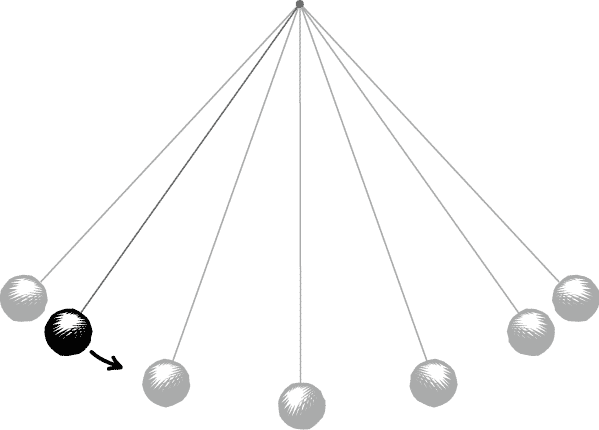
\includegraphics[width=0.8\linewidth]{Pictures/pendulum13}			
				\end{center}
			\end{column}	
			\begin{column}{.50\linewidth}
				\begin{center}
					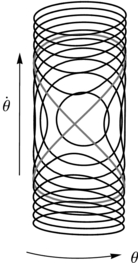
\includegraphics[width=0.45\linewidth]{Pictures/pendulum-phase-space}			
				\end{center}
			\end{column}	
		\end{columns}
		%
		\begin{defblock}[Symplectic Manifold]
			\includestandalone[width=0.95\textwidth]{Pictures/Figure_sym}	
		\end{defblock}
		%
		\begin{exblock}[$M = T^\ast Q$ is symplectic]
			$\omega = d \theta $ with
			$$ \left.\theta\right\vert_{(q,p)} (v) = p (\pi_\ast v) ~.$$
		\end{exblock}
	\end{column}
	\vrule{}
	\pause
	\begin{column}{.50\linewidth}
		\centering
		\textit{ "algebraic approach" to mechanics \dots}
		\vspace{1em}	
		\begin{defblock}[Classical Observables]
			Unital, associative, commutative algebra $C^\infty(M)$.
		\end{defblock}
		%
		\vspace{1em}
		\pause
		\begin{defblock}[Hamiltonian vector fields]
			$v_f \in \mathfrak{X}(M)$ such that:
			$$\iota_{v_f} \omega = -df \quad \text{(exact)}$$ %$\in B^1(M)$
			\small$v_f$ = \emph{Ham.v.f. pertaining to $f\in C^\infty(M)$}.
		\end{defblock}
		%
		\begin{defblock}[Poisson Algebra of Observables]
			$C^\infty(M)$ is a Poisson algebra with
			$$\{f,g\} = \iota_{v_g} \iota_{v_f} \omega = \omega(v_f,v_g) ~.$$
		\end{defblock}
	\end{column}
\end{columns}
\end{frame}
\note[itemize]{
	\footnotesize

	\item We work in the framework of multisymplectic geometry which is one of the possible generalizations of the well-established field of symplectic geometry.
	
	\item To recall what symplectic geometry is let me assume a particular point of view: mechanics.
	\\
	Idea:"
	Symplectic geometry is a branch of differential geometry studying symplectic manifolds; it originated as a formalization of the mathematical apparatus of classical mechanics and geometric optics."{\href{https://ncatlab.org/nlab/show/symplectic+geometry}{nlab}}
	
	Namely, a sym. mfd. is the geometric structure encoding the phase space of conservative, ordinary, classical, mechanical systems.
	
	\item $\theta$ = \emph{tautological 1-form}.
		$\theta$ evaluated at $p\in T^*Q$ in the fibre of $q\in Q$ and contracted with $v$ coincides with the form $p$ evaluated at $q$ and contracted with the push forward of $v$.
	
	\item We identify a special class of vector fields.
		Out of them one can define a Lie bracket.
	
	\item Poisson is a Lie algebra with the extra property of compatibility with the associative product (Leibniz rule)
}
%-------------------------------------------------------------------------------------------------------------------------------------------------





%------------------------------------------------------------------------------------------------
\begin{frame}[fragile]{MS geometry and classical field mechanics}
		Consider a smooth manifold $Y$,
		\begin{columns}
			\hfill
			\begin{column}{.5\linewidth}
				\emph{Multicotangent bundle} $\bigwedge = \bigwedge^n T^\ast Y$\\
				is naturally $n$-plectic
			\end{column}
			\begin{column}{.4\linewidth}
				\[
				\begin{tikzcd}
					\Lambda \ar[d,"\pi"'] & T \Lambda \ar[d,"T \pi"] \ar[l] \\
					Y								& T Y \ar[l]
				\end{tikzcd}	
				\]
			\end{column}
		\end{columns}
	\pause
	\begin{defblock}[Tautological $n$-form]
		$\theta \in \Omega^n(\Lambda)$ such that:
		\begin{displaymath}
		\begin{split}
			\left[ \iota_{u_1 \wedge \ldots \wedge u_n} \theta \right]_\eta 
			&= \iota_{(T \pi)_\ast u_1 \wedge \ldots \wedge (T \pi)_\ast u_n} \eta \\
			&= \iota_{u_1 \wedge \ldots \wedge u_n} \pi^\ast \eta 
			\qquad \qquad \forall \eta \in \Lambda \, , \: \forall u_i \in T_\eta \Lambda 		
		\end{split}
		\end{displaymath}
	\end{defblock}
	\vfill
	\begin{columns}
		\begin{column}{.6\linewidth}
			\begin{defblock}[Tautological (multisymplectic) (n+1)-form]
				$$\omega := d \theta$$
			\end{defblock}
		\end{column}
		\begin{column}{.4\linewidth}
		 	\begin{claimblock}$\omega$ is not degenerate.\end{claimblock}	
		\end{column}
	\end{columns}	
	\pause
	\begin{keywordblock}
		\begin{tabular}{|c|c|c|}
			\hline 
			point-particles mechanics & $\rightsquigarrow$ & classical fields mechanics \\
			%(finite discrete DOF) & & (finite dimensional continuous DOF) \\
			\hline 
			symplectic & $\rightsquigarrow$ & multisymplectic \\ 
			\hline 
			Observables (Poisson) algebra & $\rightsquigarrow$ & Observables $L-\infty$ algebra
			 \\ 
			\hline 
			Co-moment map & $\rightsquigarrow$ & Homotopy co-momentum map \\ 
			\hline 
		\end{tabular} 
	\end{keywordblock}

	
\end{frame}
\note[itemize]{
	\item This example is significant from the perspective of geometric classical field theory:
		\begin{displaymath}
			\frac{\text{classical mechanics}}{\text{symplectic geo.}} =
			\frac{\text{classical field mechanics}}{\text{multisymplectic geo.}}
		\end{displaymath}
	\item Multicotangent bundle is the \emph{Higher analogue} of the cotangent bundle.
	(but it is not yet the analogue of a \emph{phase space}.)
\item The multiphase space is the sub-bundle of $n$-forms vanishing when contracted with 2 vertical fields.
  	\item The reason why this sub-bundle has a particular role is that it can be proved to be isomorphic to a suitable dual of the first Jet bundle.
  	\item For further details see Gotay et al. \href{https://arxiv.org/abs/physics/9801019}{arXiv:physics/9801019}. For a pictorial representation of all the structures involved in the geometric mechanics of I order classical field theories see appendix, pag: \ref{frame:Gimmsy}.
}
%------------------------------------------------------------------------------------------------	
	
%------------------------------------------------------------------------------------------------
\begin{frame}{Special classes of smooth objects} 
  	\begin{columns}
		\begin{column}[t]{.42\linewidth}		
			\begin{defblock}[Hamiltonian v.f.]
				$\mathfrak{X}_{ham} =  \left\lbrace X \in  \mathfrak{X} \right\vert \left. \iota_x \omega \textrm{ exact}  \right\rbrace$ 			
			\end{defblock}
			\begin{defblock}[Multisymplectic v.f.]
				$\mathfrak{X}_{ms} =  \left\lbrace X \in  \mathfrak{X} \right\vert \left. \mathcal{L}_X \omega = 0  \right\rbrace$ 	
			\end{defblock}
		\end{column}
		\begin{column}[t]{.58\linewidth}		
			\begin{defblock}[Hamiltonian $(n$-$1)-$forms]
				\begin{displaymath}
					\Omega^{n-1}_{ham} 	:=
					\biggr\{ H \in  \Omega^{n-1} \; \left\vert \; 
					\stackanchor{$\exists X \in \mathfrak{X}_{ham}$}{: $d H = -\iota_X \omega$} \right\} 
			\end{displaymath}
			\end{defblock}		
		\end{column}
  	\end{columns}
  	%
  	\vspace{0.5em}
  	%
  	\onslide<2->{
  	\begin{columns}
		\begin{column}[t]{.5\linewidth}	
			\centering\emph{Global symmetries}
			\begin{defblock}[Multisymplectic (Lie group) action]
				$\Phi: G \circlearrowright (M, \omega)$ \emph{right action} s.t. \\
				$$\hat{\Phi}(g)_\ast \omega = \omega \quad \forall g \in G$$
			\end{defblock}
		\end{column}
		\begin{column}[t]{.5\linewidth}			
			\centering\emph{Infinitesimal symmetries}
			\begin{defblock}[Multisymplectic (Lie algebra) action]
				$V: \mathfrak{g} \rightarrow \mathfrak{X} (M)$ \emph{Lie algebra morphism} s.t. \\
				$$\mathcal{L}_{V_\xi} \omega = 0 \quad \forall \xi \in \mathfrak{g}$$	
			\end{defblock}
		\end{column}
  	\end{columns}
  	}
  	%
  	\onslide<3->{		
	  	\begin{asideblock}[Hierarchy of conserved quantities]%Shades of...
	  		\begin{table}[] % http://tablesgenerator.com/
			\begin{tabular}{lllll}
					& strictly conserved & & & $\mathcal{L}_X \alpha= 0$ \\
				$\alpha \in \Omega^\bullet$ & globally conserved & along $X \in \mathfrak{X}$ & $\Leftrightarrow$ & $\mathcal{L}_X \alpha\in B $ (exact) \\
				  & locally conserved  & & & $\mathcal{L}_X \alpha\in Z $ (closed)                                
			\end{tabular}
			\end{table}
	  	\end{asideblock}
  	}
  	
  \end{frame}
  \note[itemize]{
  	\item Exactly as it happens in symplectic geometry, fixing a smooth form $\omega$ on $M$ yields a criterion for classifying vector fields and differential forms.
  	\\(Pay attention to the sign convention in defining the Hamiltonian vector fields)
  	\item Also, we can naturally select a special class of symmetries (global and infinitesimal) which preserve the fixed multisymplectic form.
  	\item Aside, we can start to see that, in this setting, measurable quantities are not only smooth functions but also differential forms with degree greater then zero.
  	For such objects can be defined weaker notions of conservation along a flow.
  	\item The idea to consider forms of various degree as observables do not fall out of the sky. 
  		For instance in a string there will be two kind of measurable quantities: extensive observable (1-forms), like the density, and intensive observables (0-forms), like the tension. 
 		%\href{https://en.wikipedia.org/wiki/Intensive_and_extensive_properties#Intensive_properties}{(wiki link on this terminology)}
  	\item Starting from this observation we can define the space of all possible observables (see next slide).
  }
%---------------------------------------------------------------------------------------------------------------------------------------------------


%------------------------------------------------------------------------------------------------
\begin{frame}[fragile,t]{Homotopy comoment map \emph{(Callies, Frégier, Rogers, Zambon)}}
  	%
		Consider a multisymplectic action $G \circlearrowright (M, \omega)$,
		%
		\begin{defblock}[Homotopy comoment map (HCMM)]				
			Is a sequence of linear maps:
			\begin{displaymath}
				(f)  = \big\lbrace f_k: \; \Lambda^k{\mathfrak g} \to L_{k-1} \subseteq \Omega^{n-k} 
				\;\big\vert\; 0\leq k \leq n+1  \big\rbrace
			\end{displaymath}
			%
			\includestandalone[width=0.95\textwidth]{Pictures/Frame_HCMM}			
			\emph{such that:}
			\begin{itemize}
				\item $f_0 = 0 $, $f_{n+1} = 0$ %(we have tacitly set $\Lambda^{-1}(M) = 0$)
				\item<2-> $-f_{k-1} (\partial p) = d f_k (p) + \varsigma(k) \alpha^{(k)} \quad \forall (k=1,\dots n+1), \; \forall p \in \Lambda^k(\mathfrak{g})$
			\end{itemize}
		\end{defblock}
		\begin{itemize}
			\item \emph{Higher analogue} of the ordinary comoment map $f\colon \mathfrak{g}\rightarrow C^\infty(M)$.
		\end{itemize}
  \end{frame}
  \note[itemize]{
		\item Notice that a HCMM pertains to an "infinitesimal" action of ${\mathfrak g}$ on $M$ 
			with ${\mathfrak g}$ being the Lie algebra of a generic Lie group $G$, 
			acting on $M$ by $\omega$-preserving vector fields.
		\item (Not.) $ p = \xi_1 \wedge \xi_2 \wedge \dots \wedge \xi_k$, 
			then $v_p = v_1 \wedge v_2 \wedge \dots \wedge v_k$ 
			where $v_i \equiv v_{\xi_i}$ are the fundamental vector fields associated to the action $G \circlearrowright M$.
	%	\item (Notation) $\iota(v_p) \omega = \iota(v_k)\dots\iota(v_1) \omega$
	%	\item $\varsigma(k) := - (-1)^{\frac{k(k+1)}{2}}$ 
		\item (Recall) $\alpha^{(k)}:= \iota(v_p) \omega = \iota(v_k)\dots\iota(v_1) \omega$
		\item $\partial \equiv \partial_k:  \Lambda^{k} {\mathfrak g} \to \Lambda^{k-1} {\mathfrak g}$  is the usual Eilenberg-Chevalley complex boundary operator (see appendix, pag: \ref{frame:CE-complex});
		\item The definition tells us that the {\it closed} forms
			$$\mu_k := f_{k-1} (\partial p) +  \varsigma(k) \iota(v_p) \omega 	$$
			must actually be {\it exact}, with potential $-f_k(p)$.  	
		\item The last equation tells us that an HCMM is not a chain complex morphism but is rather a chain complex homotopy between 0 and the multicontraction $\alpha$ (is a chain map by lemma 2.18 \cite{Ryvkin2016}).
		\item An HCMM is a L-$\infty$ morphism 
		$(f):\mathfrak(g)\rightarrow L(M)$ s.t. 
		$d f_1(\xi) = -\iota_{v_\xi} \omega$.\\
		\footnotesize{(Compare with the definition of ordinary comoment map: \\Lie algebra morphism 
		$J:\mathfrak(g)\rightarrow C^\infty(M)$ s.t. $ d J(\xi) =  -\iota_{v_\xi} \omega$)}
		
  }
%------------------------------------------------------------------------------------------------

%------------------------------------------------------------------------------------------------
\begin{frame}{Geometry of symmetries}\label{frame:geometrysymmetries}
	Basic mechanical structures are encoded in geometry. but there is another complementary geometrical property that's natural in physics: symmetry!
	\begin{alertblock}{Upshot}
		Continous symmetries are described by actions of a Lie group on $M$.
	\end{alertblock}
	\begin{block}{Noether}
		Presence of symmetries $\quad \Rightarrow \quad$ existence of conserved quantities.
	\end{block}	
	\begin{block}{Key concept:}
		Noether current are encoded in a \emph{moment map}  $\mu :M \rightarrow \mathfrak{g}^*$ (the dual of the comoment map $f$. 
	\end{block}
  \begin{columns}[T]
   	\begin{column}{.6\textwidth}
			\begin{block}{Symplectic reduction:}
			\begin{itemize}
				\item System dynamics should be restricted to level set of conserved observables in order to efficiently store dynamical properties.
				\item Under certain assumptions, $\mu^{-1}( 0 )/G$ is a symplectic manifold with an "induced" symplectic structure.
			\end{itemize}
			\end{block}
    \end{column}
    \begin{column}{.4\textwidth}	
			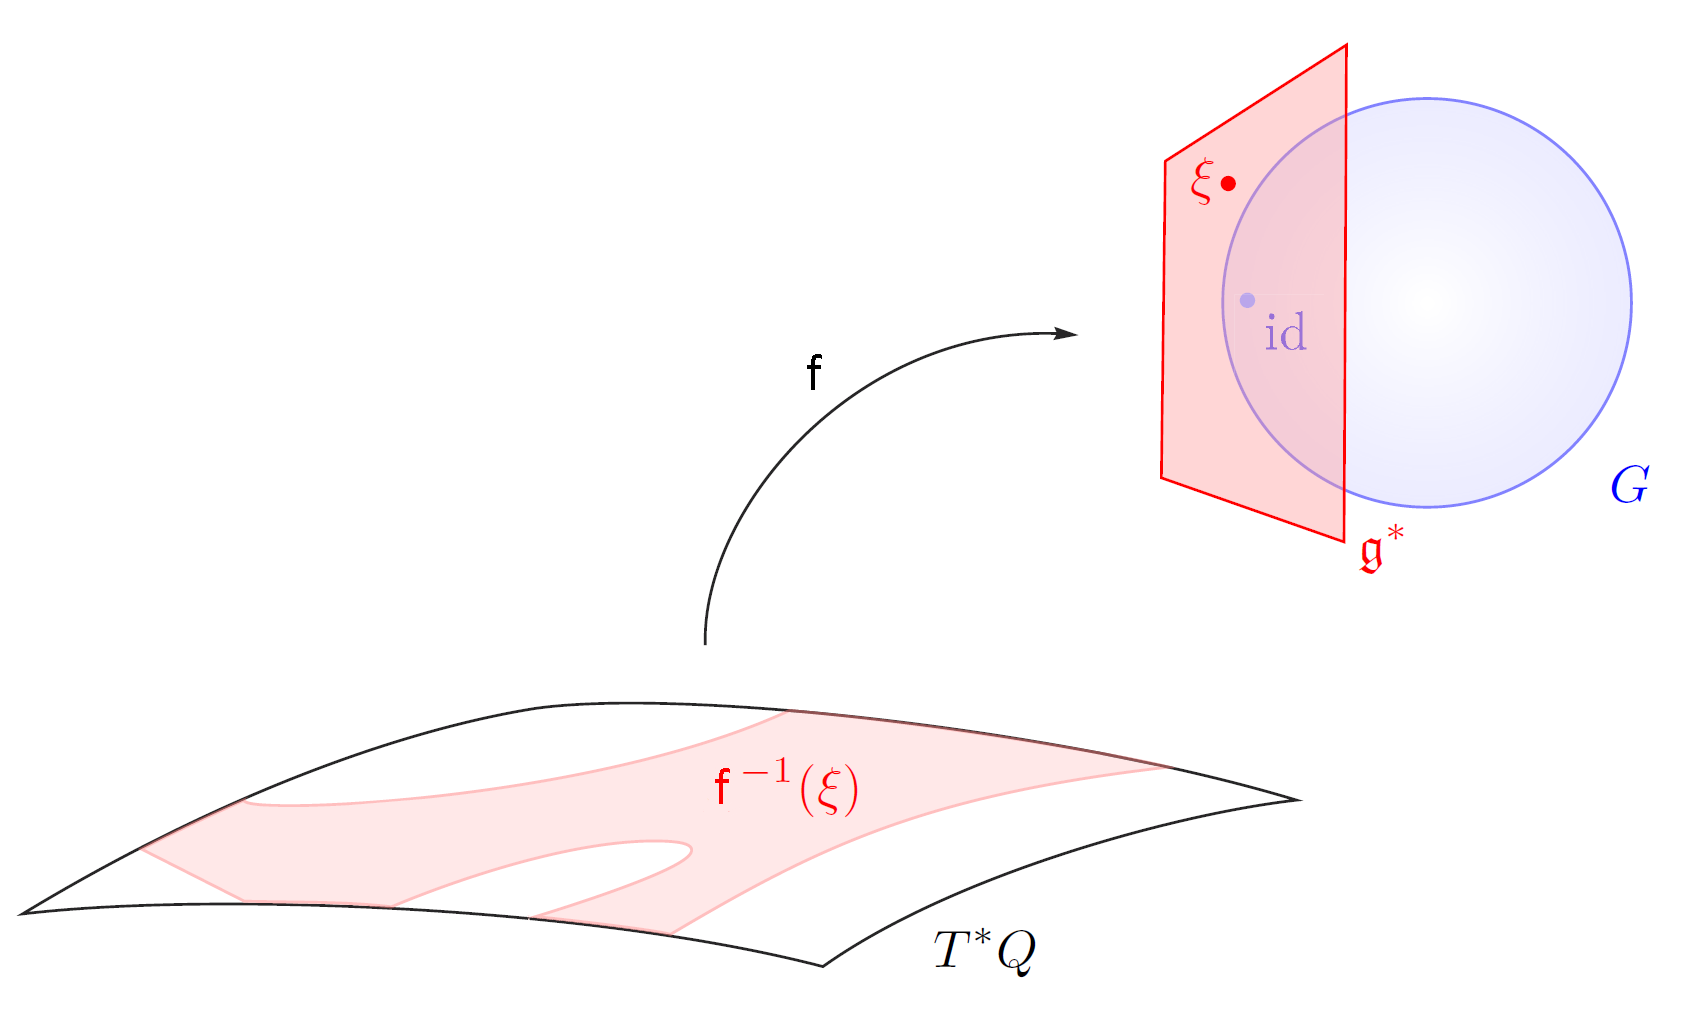
\includegraphics[width=\textwidth]{Pictures/Reduction} 
  	\end{column}
	\end{columns}			
\end{frame}
%------------------------------------------------------------------------------------------------

%##################################################################################
\section{Work Done with Mauro}
%##################################################################################

%------------------------------------------------------------------------------------------------
  \begin{frame}{Explicit Construction of the HCMM for $SDiff_0 \circlearrowright (\mathbb{R}^3,\nu)$}\label{frame:explicithcmm}
	\begin{columns}
		\begin{column}[c]{.5\linewidth}
		  	\begin{itemize}
		  		\item The observables are  $$L= \Omega^1_{\textrm{ham}}(\mathbb{R}^3)\oplus\Omega^0(\mathbb{R}^3)$$
		  		\item HCMM consists of a pair of functions:
					\begin{align*}
						f_1 &\colon \mathfrak{g} \rightarrow \Omega^1_{\textrm{ham}}(\mathbb{R}^3) \\
						f_2 &\colon \mathfrak{g}\wedge\mathfrak{g} \rightarrow C^\infty(\mathbb{R}^3)
					\end{align*}	
		  	\end{itemize}
		\end{column}	
	  	\hfill  	
		\begin{column}[c]{.5\linewidth}
  		\includestandalone[width=\textwidth]{./Pictures/Figure_Euclid_Trigger}
 	 	\end{column}
 	 \end{columns}
 	\begin{columns}
		\begin{column}[c]{.8\linewidth}
		 	 \begin{itemize}
				\item Satisfying the following system:
					\begin{displaymath}
						\begin{cases}
							\textrm{d} f_1(\xi) = \iota_\xi \nu = -\alpha^1(\xi) \\
							\textrm{d} f_2(\xi_1 \wedge \xi_2) = f_1\left([\xi_1,\xi_2]\right) - \iota_{\xi_2}\iota_{\xi_1} \nu 
							 := \mu_2(\xi_1,\xi_2)\\
							f_2\left(\partial \xi_1 \wedge \xi_2 \wedge \xi_3 \right) = \iota_{\xi_3}\iota_{\xi_2}\iota_{\xi_1} \nu
						\end{cases}
					\end{displaymath}
				\item Results: 
					\begin{align*}
						f_1 &= \flat \circ {\rm curl}^{-1} \\
						f_2 &= {\rm grad}^{-1} \circ \sharp \circ \mu_2  
					\end{align*}	
		 	 \end{itemize}
 	 	\end{column}
		\begin{column}[c]{.2\linewidth}
 	 	\end{column}
 	 \end{columns}
  \end{frame}
	\note[itemize]{
		\tiny
		\item On the left there is the part of the Chevalley-Eilemberg complex that interact with the L-$\infty$ algebra of observables.
		\item On the right there is the whole de Rham complex of the manifold $M=\mathbb{R}^3$.
		\item Even if only $\Omega^1$ and $\Omega^0$ take part in the definition of a $HCMM$, the Riemmanian structure determine a correspondence with the rest of the de Rham complex.
		\item In order to give an HCMM for this action is necessary to give a solution of the system of 3 equations below.
		\item Recall: $ 	\ast: \Omega^k \rightarrow \Omega^{n-k}$ where $\ast \sigma$ is defined as the unique form such
		 that $ \omega \wedge \ast \sigma = \nu \lbrace \omega, \sigma \rbrace$ where 
		 $\langle,\rangle$ is the inner product on forms induced by the metric.
		\item Be aware of the sloppy notation: 
						the inverse of vector calculus differential operators are to be thought as their green operators.(There is no unique inverse of the curl!)
			Also, the second one, is the operation of taking a primitive $f_2={\rm d}^{-1} \circ \mu_2 $.
		\item UPSHOT: 
			\begin{itemize}
				\item We described a natural example motivated by physics,( momenta are related to vortices $\Leftarrow$).
				\item Transgression to loop spaces yields something already known in the context of fluid dynamics;		
				\item exemplified the generaf phenomenon that multisymplectic manifolds appear to be a \alert{"finite dimensional"} object able to encode features of \alert{"infinite dimensional"} mechanical systems.
			\end{itemize}
	}  
%---------------------------------------------------------------------------------------------------------------------------------------------------

%---------------------------------------------------------------------------------------------------------------------------------------------------
\begin{frame}[fragile]{Hydrodynamics interpretation}\label{frame:hydrointerpretation}
		Consider the loop spaces $L{\mathbb R}^3$,\\
		%
		\begin{propblock}[HCMM for $G\circlearrowright(\mathbb{R}^3,\nu)$ induces \\an ordinary co-mo.map for $G\circlearrowright (LS,\nu^{\ell})$]
			The HCMM $f \colon \mathfrak{g} \to L_{\infty}(\mathbb{R}^3,\nu)$ previously given
			\emph{transgresses}	 to
			\begin{displaymath}%\tag{Arnol'd-Marsden-Weinstein\\ hydrodynamical co-momentum map}
				\begin{tikzcd}[column sep= small,row sep=0ex]
					\lambda \colon& \mathfrak{g}	\arrow[r]& C^\infty(LS) \\
					& {\mathbf b}	\arrow[r, mapsto]
					& \displaystyle \biggr( \gamma \mapsto \lambda_b(\gamma) = - \oint_{\gamma} f_1({\mathbf b})  \biggr)	
				\end{tikzcd}	
			\end{displaymath}
			that is a  moment map for the induced action $G$ on the pre-symplectic loop space $(LM,\nu^{\ell})$. (Smooth space in the sense of Brylinski)
		\end{propblock}
		\begin{itemize}
			\item $\lambda$ corresponds to \emph{Arnol'd-Marsden-Weinstein hydrodynamical co-momentum map}  defined on $\infty$-dim. manifolds.
			\item<2-> $\Lambda = \left\lbrace \lambda_{\mathbf b} \right\rbrace_{{\mathbf b}\in\mathfrak{g}}$ is, up to sign, the {\it Rasetti-Regge current algebra}
			\item<3-> There is a naturally defined {\it Poisson brackets} on $\Lambda$:
				\begin{displaymath}
					\{ f_1({\mathbf b}), f_1({\mathbf c}) \} (\cdot):= \iota_{\mathbf c} \iota_{\mathbf b} \nu (\cdot)=
						\nu({\mathbf b}, {\mathbf c}, \cdot) = f_1([{\mathbf b},{\mathbf c}])
					-df_2 ({\mathbf b} \wedge {\mathbf c})
				\end{displaymath}
				\centering\footnotesize(Note: $\lambda$ is (infinitesimally) $G$-equivariant, i.e. $	\{\lambda_{\mathbf b}, \lambda_{\mathbf c} \} = \lambda_{[{\mathbf b}, {\mathbf c}]}$)
		\end{itemize}

    
\end{frame}
\note[itemize]{
  	\item[ ] \textbf{How all of this is relevant in Hydrodynamics?}
  	\item The loop space is the manifold, in the sense of Brylinsky, consisting of all smooth loops in ${\mathbb R}^3$.
  	\item Transgression can be seen as a pull-back along the evaluation map 
  		$${\rm ev}: L{\mathbb R}^3 \times {\mathbb R} \ni (\gamma, t) \mapsto \gamma(t) \in {\mathbb R}^3$$
  		  	For further details see appendix, pag: \ref{frame:LoopSpacesTransgression}.
  	\item Note that the (RR) current pertaining to ${\mathbf b} \in {\mathfrak g}$  is independent of the choice of $B$.
  			See appendix, pag: \ref{frame:RRcurrents} for other informations on this concept or \cite{Rasetti1975},\cite{Penna1992} for a deeper account.
  	\item In \cite{Callies2016} is proved a general result asserting that, roughly speaking,
			homotopy co-momentum maps transgress to homotopy co-momentum maps on loop (and even mapping) spaces. Further details in appendix, pag: \ref{frame:TransgressionHCMM}.
	\item Actually, the ansatz for $f_1$ term in the previous construction has been precisely motivated by this phenomenon. 
}
%------------------------------------------------------------------------------------------------

\begin{frame}{Hamiltonian forms related to a n-link}\label{frame:msknots1}

		
  	\onslide<1->{
  	\begin{columns}
		\begin{column}[c]{.7\linewidth}	
				Let $ L = \cup_{i=1}^n L_i$ be an oriented link in ${\mathbb R}^3$ 
				\\(components $L_i$, $i=1,\dots,n$ required to be  {\it trivial} knots)	
		\end{column}
		\begin{column}[c]{.25\linewidth}	
			\centering{
			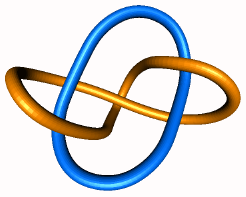
\includegraphics[width=0.75\linewidth]{./Pictures/Whiteheadlink}
			}
		\end{column}
  	\end{columns}
  	}
		%
  	\onslide<2->{
  	\begin{columns}
		\begin{column}[t]{.5\linewidth}	
			\begin{defblock}[Vorticity 2-form]
				$$
				\omega_{L} := \sum_{i=1}^n \omega_{L_i}, \qquad d\omega_L = 0
				$$
				($\omega_{ L_i}$ = Poincar\'e dual associated to $L_i$)
			\end{defblock}
		\end{column}
		\begin{column}[t]{.5\linewidth}	
			\begin{defblock}[Velocity 1-form]
				$$
 					v_{ L} = \sum_{i=1}^n v_{L_i}, \qquad \qquad  dv_{L} = \omega_{ L}
				$$
				($v_{L_i} := \omega_{{\mathfrak a}_i}$ = Poincar\'e dual  of a disc ${\mathfrak a}_i$ 
				bounded by 	$L_i$ \footnotesize{(Seifert surface)}) 
			\end{defblock}						
		\end{column}
  	\end{columns}
  	}
  	%
  	\begin{columns}
		\begin{column}[t]{.3\linewidth}	
  		\onslide<2->{
  			\center
  			\vspace{-4ex}
				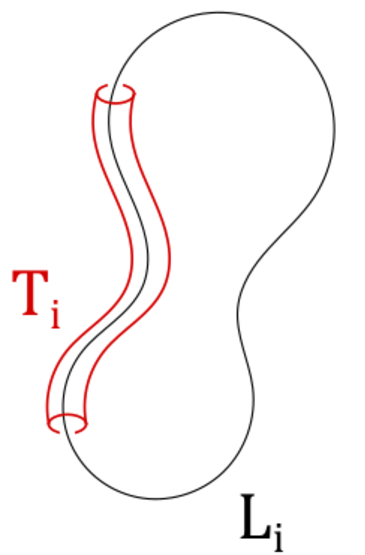
\includegraphics[width=0.6\linewidth]{./Pictures/tubes}
	  	}			
		\end{column}
		\begin{column}[t]{.7\linewidth}	
  	\onslide<3->{
			\begin{propblock}[$v_{L}$ is a {\it Hamiltonian 1-form}]
				For each component $L_i$, the Hamiltonian vector field $\xi_{L_i}$ of 
				$v_{L_i}$ is $-\alpha^{-1}(\omega_{L_i})$.
				\\
				Explicitly, one has 
				\begin{displaymath}
					dv_L + \sum_{i=1}^n\iota_{\xi_{L_i}} \nu = 0 				
				\end{displaymath}
			\end{propblock}  	
  	}				
		\end{column}
  	\end{columns}
\end{frame}
\note[itemize]{
	\item $\omega_{ L_i}$ denote the Poincar\'e (or Thom) dual (class) associated to $L_i$: they are 2-forms localized in a 
 cross-section of a  suitable tubular neighbourhood $T_i$ around $L_i$ - with total fibre integral equal to one, or, as currents, 2-forms which are $\delta$-like on $L_i$
 
	\item $v_{L_i} := \omega_{{\mathfrak a}_i}$ is the Poincar\'e dual (class) of a disc ${\mathfrak a}_i$ bounding
$L_i$ (a Seifert surface for the trivial knot $L_i$). Precisely:
$$
\partial {\mathfrak a}_i = L_i, \qquad \qquad dv_{L_i} = d\omega_{{\mathfrak a}_i} = \omega_{L_i} = \omega_{\partial {\mathfrak a}_i},
$$
	\item
		Velocity 1-forms $v_i$ correspond (upon approximation of the associated Euler equation) to the so-called LIA (Linear Induction Approximation) or  {\it binormal evolution}
		of the ``vortex ring" $L_i$ (``orthogonal" to the discs ${\mathfrak a}_i$.
		
	\item Everything is up to choices of tubular neighbourhoods, Seifert surface and specific Poincar\'e dual.


}
%------------------------------------------------------------------------------------------------


%------------------------------------------------------------------------------------------------
\begin{frame}{Relation with Gauss linking number}\label{frame:msknots2}
		%
		\vspace{-2.5ex}
		%
  	\begin{columns}
		\begin{column}[t]{.5\linewidth}	
			\begin{defblock}[Chern-Simons 3-form]
				$$
					CS({L}) :=  v_{L} \wedge  \omega_{ L} 
				$$
			\end{defblock}
		\end{column}
		\begin{column}[t]{.5\linewidth}	
			\begin{defblock}[Helicity]
				$$
 					{\mathcal H}(L) = \int_{\mathbb{R}^3} CS({L})
				$$
			\end{defblock}						
		\end{column}
  	\end{columns}
	\pause
	\begin{propblock}[
		Choosing a parametrization $\mathbf{r}_i$ (in standard coordinates) for each $L_i$ 
		\begin{displaymath}
			{\mathcal H}(L)  = 
			\sum_{i,j=1}^n
			\,\frac{1}{4\pi}
			\oint_{\gamma_i}\oint_{\gamma_j}
			\frac{\mathbf{r}_i - \mathbf{r}_j}{|\mathbf{r}_i - \mathbf{r}_j|^3}
			\cdot (d\mathbf{r}_i \times d\mathbf{r}_j) =
			\sum_{i,j=1}^n \ell(i,j)
		\end{displaymath}
			$\bullet$ $\ell(i,j) = \ell(j,i)$ : Gauss linking number of components $L_i$ and $L_j$ if $i\neq j$\\
			$\bullet$ $\ell(j,j)$ : {\it framing} of $L_j$\\ 
			\phantom{-------}\footnotesize{ (i.e. $\ell(L_j, L_j^{\prime})$ with $L_j^{\prime}$ being a section of the normal bundle of $L_j$.)}\normalsize

		]
	\pause
  	\begin{columns}
		\begin{column}[c]{.7\linewidth}	
		\underline{Sketch}: Cosider a Hopf Link
			\begin{displaymath}
				L(C,C') = \eta_C \wedge \eta_{\Sigma'} + \eta_{C'} \wedge \eta_\Sigma =
				\eta_{P'} + \eta_{P}
			\end{displaymath}
		\end{column}
		\begin{column}[c]{.25\linewidth}	
			\centering{
			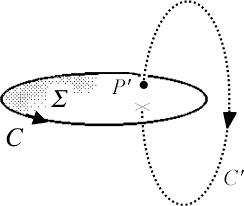
\includegraphics[width=0.75\linewidth]{./Pictures/GaussLink}
			}
		\end{column}
  	\end{columns}
			Therefore $\int L(C,C') = \ell(C,C')$ 
			algebraically counts crossings of a component with a Seifert surface of a different one.			%sign is given by the orientation.
		\end{propblock}
		
\end{frame}
\note[itemize]{
	\item Our previous construction is heavily dependent on a lot of choices 
	but we end up with a quantity that only depends on the starting n-link.
	\item ${\mathcal H}(L)$ is invariant under ambient isotopies.\\
	However, non ambient isotopic links do not necessarily yield different linking numbers
	(it is not an universal invariant!).
  	\begin{columns}
		\begin{column}[c]{.5\linewidth}	
			\centering{
			\includegraphics[width=0.5\linewidth]{./Pictures/UnknotsGauss}
			}
		\end{column}
		\begin{column}[c]{.5\linewidth}	
			\centering{
			\includegraphics[width=0.35\linewidth]{./Pictures/WhiteheadGauss}
			}
		\end{column}
  	\end{columns}	
	\item
		\begin{displaymath}
	\begin{split}
		\text{link}(\gamma_1,\gamma_2) &=\,\frac{1}{4\pi}
		\oint_{\gamma_1}\oint_{\gamma_2}
		\frac{\mathbf{r}_1 - \mathbf{r}_2}{|\mathbf{r}_1 - \mathbf{r}_2|^3}
		\cdot (d\mathbf{r}_1 \times d\mathbf{r}_2)\\[4pt]
		 &= \frac{1}{4\pi}\int_{S^1 \times S^1} \frac{\text{det}(\dot{\gamma_1}(s),
	 \dot{\gamma_2}(t),\gamma_1(s)-\gamma_2(t))}{|\gamma_1(s)-\gamma_2(t)|^3}\, ds \, dt
	\end{split}
	\end{displaymath}
}
%------------------------------------------------------------------------------------------------

%##################################################################################
\section{Work Done with Leonid}
%##################################################################################
%-------------------------------------------------------------------------------------------------------------------------------------------------
\begin{frame}[fragile]{Cohomological obstructions for compact groups}\label{frame:cohomologicalproposition}
	Let $\vartheta:G\times M\to M$ be a compact Lie group acting on a pre-multisymplectic manifold, preserving the pre-multisymplectic form $\omega$. 
	%
	\begin{propblock}
		[ $\exists$ (HCMM) $ 
			~\Leftrightarrow~ 
			\lbrack\vartheta^*\omega-\pi^*\omega\rbrack=0\in H^{n+1}(G\times M)$]
		Based on the sequence of isomorphisms:
		\begin{center}
			\begin{tikzcd}
	 			\Omega^\bullet(M,\vartheta) \ar[d,"\vartheta^\ast-\pi^\ast"] &\quad
				 & H_\text{dR}(M) \ar[d,"\vartheta^\ast-\pi^\ast"]  
				 & \lbrack \omega \rbrack \ar[d,mapsto]
				 \\ 
				 \Omega^\bullet(G\times M, r\times id) \ar["\cong",leftrightarrow]{d} &\quad
				 & H_\text{dR}(G\times M) \ar[leftrightarrow,"\cong"]{d}[swap]{\text{\tiny (K\"unneth)}} 
				 & \lbrack \vartheta^\ast \omega - \pi^\ast \omega \rbrack \ar[ddd,mapsto]
				 \\ 
				 \Omega^\bullet(G,r) \otimes \Omega^\bullet(M) \ar["\cong",leftrightarrow]{d}[swap]{} &\quad
				 & H_\text{dR}(G) \otimes  H_\text{dR}(M) \ar[d,"\cong",leftrightarrow]
				 \\ 
				 \Lambda^\bullet \mathfrak{g}^* \otimes \Omega^\bullet(M)\ar["\cong",leftrightarrow]{d} &\quad
				 & H_\text{CE}(\mathfrak{g}) \otimes  H_\text{dR}(M) 
				 \ar["\cong",leftrightarrow]{d} & 
				 \\
				 C_\mathfrak{g}^\bullet \oplus ( \mathbb{R}\otimes \Omega^\bullet(M))&\quad 
				 & H(C_\mathfrak{g}^\bullet)\oplus H_\text{dR}(M)
				 & \lbrack \tilde{\omega}\rbrack
			\end{tikzcd}
		\end{center}						
	\end{propblock}
\end{frame}
%-------------------------------------------------------------------------------------------------------------------------------------------------


%------------------------------------------------------------------------------------------------
\end{document}